        \documentclass{standalone}
        \usepackage{../BlogTikz}
        \begin{document}

\tikzset{snake it/.style={decorate, decoration={snake, amplitude=3mm, segment length=15mm, post length=0pt}}}
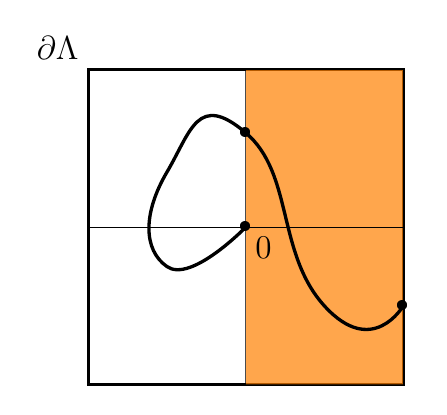
\begin{tikzpicture}[scale=1]
\tikzstyle{every node}=[font=\small]
	\draw[very thick] (-2,-2) to (2,-2) to (2,2) to (-2,2) to cycle;
	\filldraw[draw=black,fill=orange, opacity=0.7] (0,-2) to (2,-2) to (2,2) to (0,2) to cycle;
	\draw (-2,0) to (2,0);
	\node[above left] at (-2,2) {\large$\partial\Lambda$};

	\draw[very thick] plot [smooth, tension=1.1] coordinates {(0,0) (-1,-0.5) (-1,0.7) (0,1.2) (1,-1) (2,-1)};
	\node at (0,0) {\textbullet};
	\node[below right] at (0,0) {\large$0$};
	\node at (0,1.2) {\textbullet};
	\node at (2,-1) {\textbullet};
\end{tikzpicture}
        \end{document}
